%%%%%%%%%%%%%%%%%%%%%%%%%%%%%%%%%%%%%%%%%%%%%%%%%%%%%%%%%%%%%%%%%%%%%
\newcommand{\AuthorA}{Chlo� Pasturel$^1$}
\newcommand{\AuthorB}{Jean-Bernard Damasse$^1$}%
\newcommand{\AuthorC}{Anna Montagnini$^1$}%
\newcommand{\AuthorD}{Laurent U.~Perrinet$^1$}%

\newcommand{\Address}{$^1$Institut de Neurosciences de la Timone, CNRS / Aix-Marseille Universit� - Marseille, France}%

%\newcommand{\Website}{http://invibe.net/LaurentPerrinet}%
%\newcommand{\Email}{Laurent.Perrinet@univ-amu.fr}%

\newcommand{\Title}{Estimating and anticipating a dynamic probabilistic bias in visual motion direction}
%\newcommand{\Conference}{GDR Vision 2017 / Lille, France \\
%Acknowledgments : ANR grant <<Reinforcement and Eye Movements>> \textbf{ANR-13-APPR-0008-02}}%

\newcommand{\Conference}{\textbf{GDR Vision 2017}, Lille, France \\\\\\\\\\\\\\\\\\\\\\\\\\\\\\\\\\\\\\\\\\\\\\\\\\\\\\\\\\\\\\\\\\\\\\\\\\\\\\\\\\\\\\\\\\\\\\\\ Acknowledgments : ANR grant <<Reinforcement and Eye Movements>> \textbf{ANR-13-APPR-0008-02}}
%%%%%%%%%%%%%%%%%%%%%%%%%%%%%%%%%%%%%%%%%%

\documentclass[profile,final,english, draft
]{sciposter}%landscape,french]{sciposter}% ,draft]{sciposter}% 
\usepackage{babel}
% MATHS (AMS)
\usepackage{amsmath}
\usepackage{amsfonts} 
\usepackage{amssymb}
\usepackage{amsthm}
\newtheorem*{thm}{Proposition}


%% ========  polices de caracteres =============
\usepackage[T1]{fontenc}% 
\usepackage{lmodern}%
\usepackage{t1enc}
\usepackage{ragged2e}
%============ graphics ===================
\usepackage[pdftex]{graphicx}% 
\DeclareGraphicsExtensions{.pdf,.png, .jpg}%
\graphicspath{{./figures/}}%
%\usepackage[numbers,comma,sort&compress,round]{natbib} %
\usepackage[%style=nature,
maxcitenames=2,
maxnames = 2,
firstinits=true,
uniquename=init,
sorting=none,
url=false,
isbn=false,
eprint=false,
texencoding=latin1,
bibencoding=utf8,
autocite=superscript,
backend=biber,
%articletitle=false
]{biblatex}%
%%%%%%%%%%%%%%%%%%%%%%%%%%%%%%
%% OPTIONAL MACRO FILES
%\usepackage{tikz,tkz-euclide} \usetkzobj{all} % loading all objects
%\usetikzlibrary{positioning} \usetikzlibrary{calc}
%\usepackage{sfmath}
%============ hyperref ===================
\usepackage[unicode,linkcolor=red,citecolor=red,filecolor=black,urlcolor=red,pdfborder={0 0 0}]{hyperref}%
\hypersetup{%
pdftitle={\Title},%
pdfauthor={\AuthorA},%< \Email > \Address},%
pdfsubject={\Conference}%
}%
\usepackage{color,multicol}%
%%============= margins ==================
\setlength{\columnseprule}{.05mm}
\makeatletter
\renewcommand{\section}{\@startsection
        {section}%              % the name 
        {1}%                    % the level
        {0mm}%                  % the indent
        {1\baselineskip}%      % the beforeskip
        {1mm}%                  % the afterskip
        {\LARGE\color{red}\bfseries}}% % the style
\renewcommand{\subsection}{\@startsection
        {subsection}%              % the name 
        {2}%                    % the level
        {0mm}%                  % the indent
        {0.5\baselineskip}%      % the beforeskip
        {1mm}%                  % the afterskip
        %{\large\color{DarkRed}\bfseries}}% % the style
        {\normalsize\color[rgb]{0.4,0,0}\bfseries}}% % the style
        
\makeatother
%%%%%%%%%%%%%%%%%%%%%%%%%%%%%%%%%%%%%%%%%%%%%%%%%%%%
%%%                mycaption                     %%%
%%%%%%%%%%%%%%%%%%%%%%%%%%%%%%%%%%%%%%%%%%%%%%%%%%%%
%\newcounter{figure}
\setcounter{figure}{1}
\newcommand{\mycaption}[1]{
  \vspace{0.5cm}
  \begin{quote}
    {{\sc Figure} \arabic{figure}: #1}
  \end{quote}
  \vspace{1cm}
  \stepcounter{figure}
}%
%
%%%%%%%%%%%%%%%%%%%%%%%%%%%%%%%%%%%
% sciposter defs
\renewcommand{\titlesize}{\Huge}
\leftlogo[1.2]{logo_INT}
\title{\Title}%
\author{\AuthorA, \AuthorB,  \AuthorC,  \AuthorD}%{\large}%
\institute{\Address}%\scriptsize
\rightlogo[1.2]{logo_CNRS-AMU}
\conference{\Conference}





\setlength{\columnseprule}{0pt}
%%%%%%%%%%%% Her begynner selve dokumentet %%%%%%%%%%%%%%%
\begin{document}%
\maketitle%
\begin{multicols}{3}
%%%%%%%%%%%%%%%%%%%%%%%%%%%%%%%%%%%%%%%%%%%%%%%%%%%%%%%%%%%%%%%%
%%% Abstract
%\begin{abstract}
%\end{abstract}


%\columnbreak

\section*{Problematic}

Humans are able to accurately track a moving object with a combination of saccades and smooth eye movements. These movements allow us to align and stabilize the object on the fovea, thus enabling high-resolution visual analysis. When predictive information is available about target motion, anticipatory smooth pursuit eye movements (aSPEM) are efficiently generated before target appearance, which reduce the typical sensorimotor delay between target motion onset and foveation. It is generally assumed that the role of anticipatory eye movements is to limit the behavioral impairment due to eye-to-target position and velocity mismatch.

By manipulating the probability for target motion direction we were able to bias the direction and mean velocity of aSPEM, as measured during a fixed duration gap before target ramp-motion onset. This suggests that probabilistic information may be used to inform the internal representation of motion prediction for the initiation of anticipatory movements.

\begin{tabular}{cc} 
    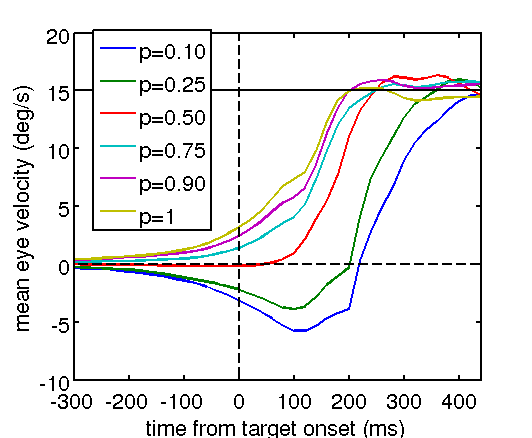
\includegraphics[width=.5\columnwidth]{image_anna_1} & 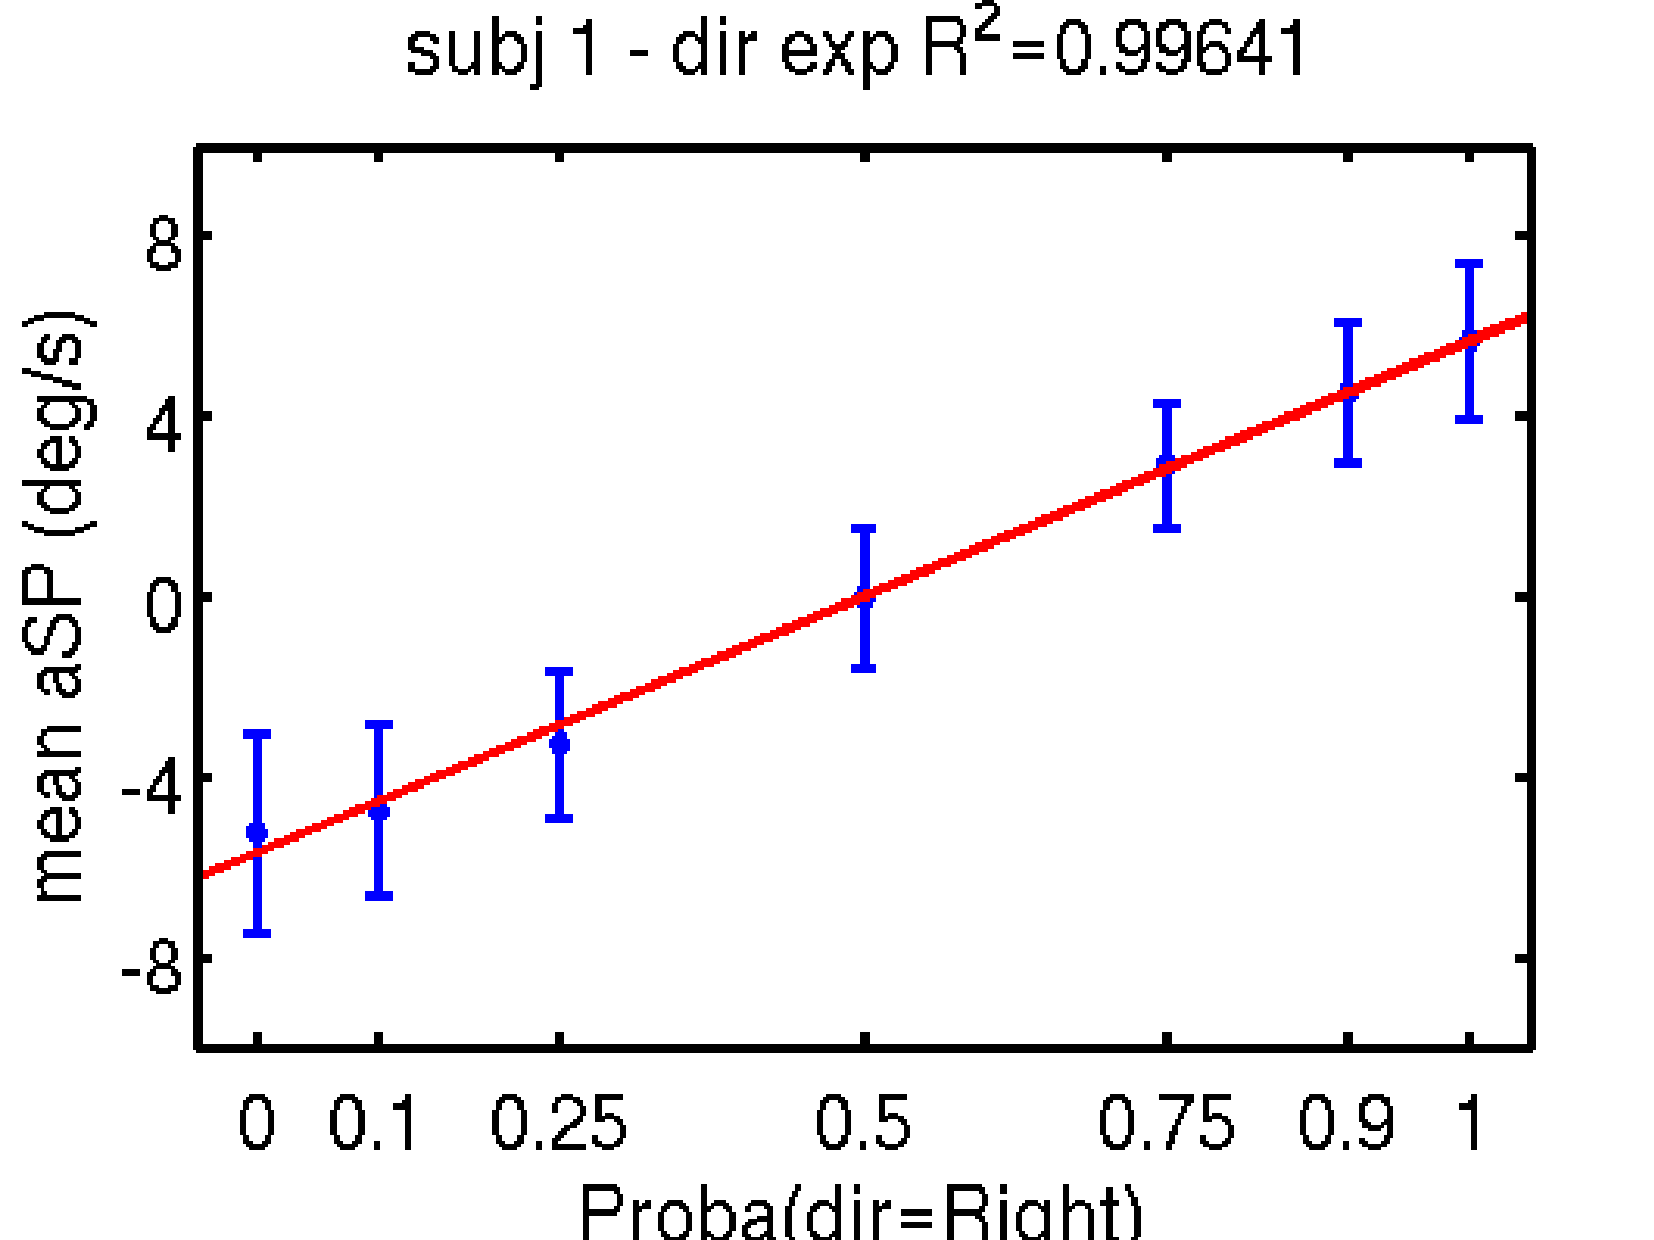
\includegraphics[width=.5\columnwidth]{image_anna_2}
\end{tabular}

However, such estimate may become particularly challenging in a dynamic context, where the probabilistic contingencies vary in time in an unpredictable way. In addition, whether and how the information processing underlying the buildup of aSPEM is linked to an explicit estimate of probabilities is unknown.


\section*{Material and Method}

In order to answer these questions we have set up an experiment comprising 3 blocks of 200 trials. For each trial a target makes a move to the left or right. The probability of this motion varied randomly in the same block.

\begin{center} 
    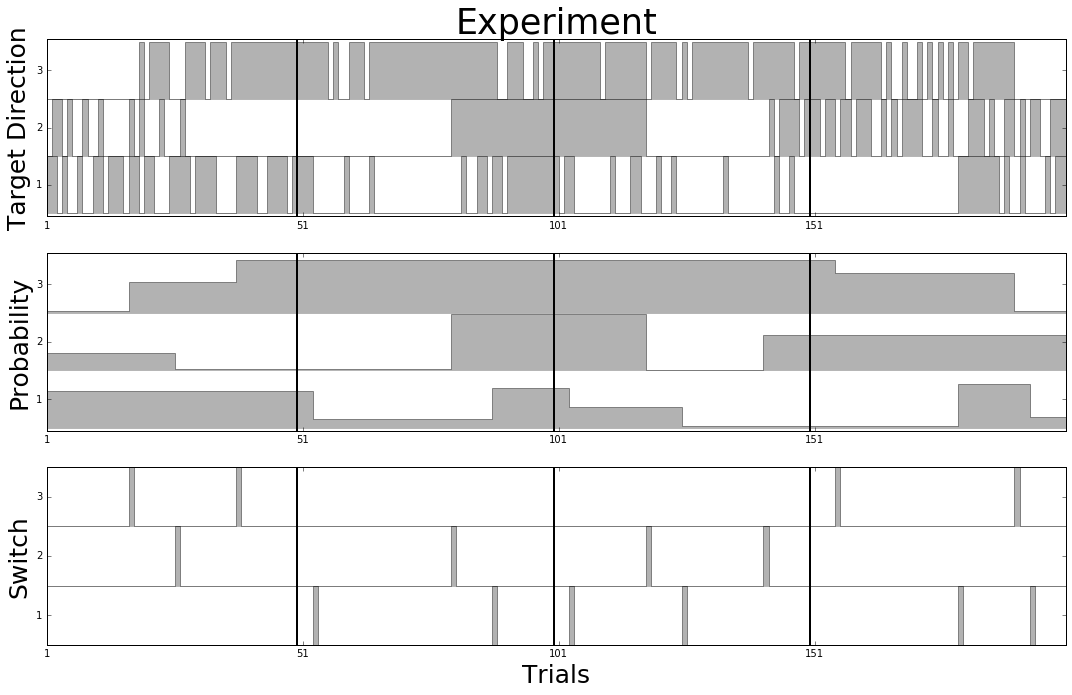
\includegraphics[width=1\columnwidth]{exp}
\end{center}

We asked subjects to do two tasks :

\begin{itemize}\setlength{\itemsep}{0ex}
\item a <<Bet>>
\item a <<recording>>
\end{itemize}


\subsection*{<<Bet>>}
In this first part, the subjects must simply answer, by adjusting a cursor on the screen, before each trial at the question \textit{<<At what point are you sure that the target will go left or right?>>}

\subsection*{<<Recording>>}
Then we recorded their eye movements when they were tracking the target's motion that same sequence.
\section*{Results}

\subsection*{<<Bet>>}

Example of results obtained during the bet :

\begin{center} 
    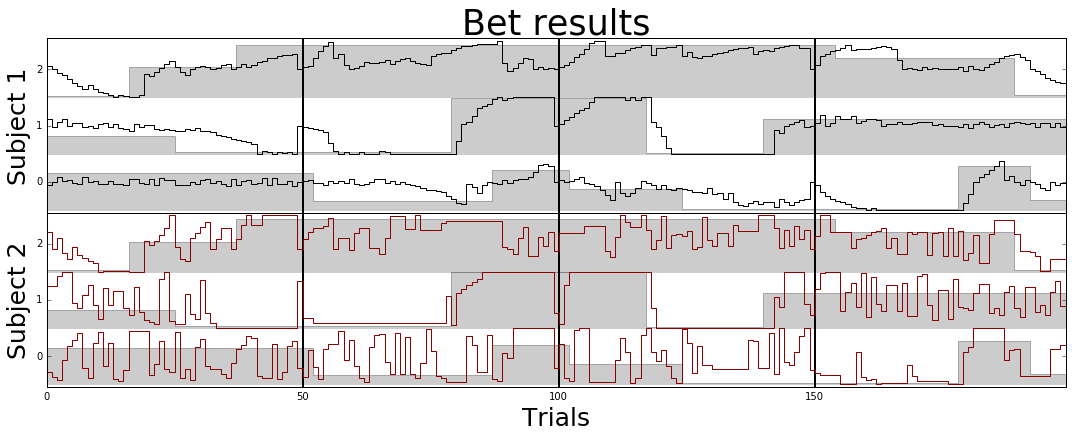
\includegraphics[width=1\columnwidth]{results_pari}
\end{center}

Comparison of probabilities bet with the real probability:

\begin{center}
    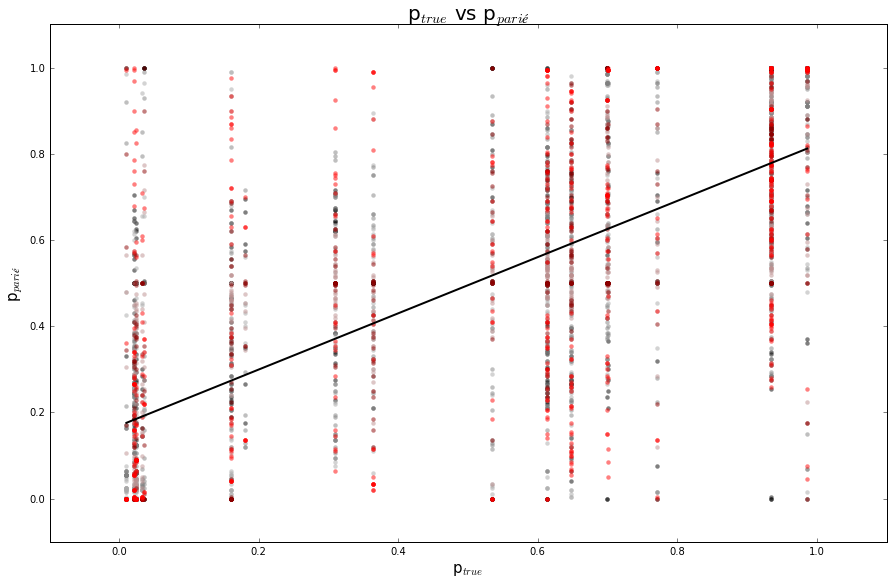
\includegraphics[width=1\columnwidth]{p_true--p_parie}
\end{center}

\subsection*{<<Recording>>}

In order to extract the relevant parameters of the oculomotor responses, we developed new tools based on best-fitting procedure
of predefined patterns : \textbf{the typical smooth pursuit velocity profile}.

\begin{center} 
    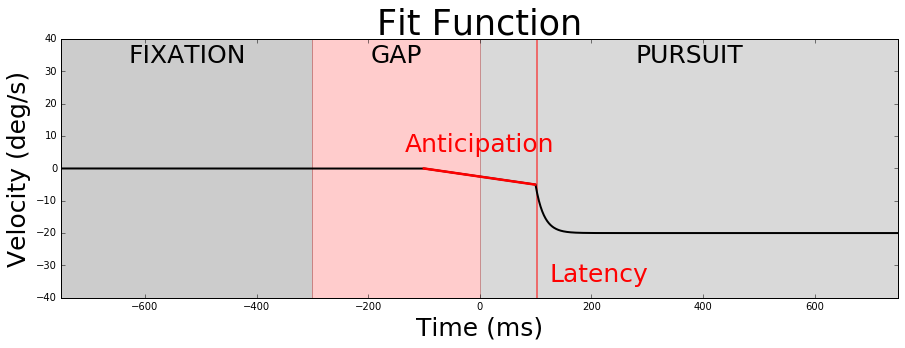
\includegraphics[width=1\columnwidth]{Fonction_Fit}
    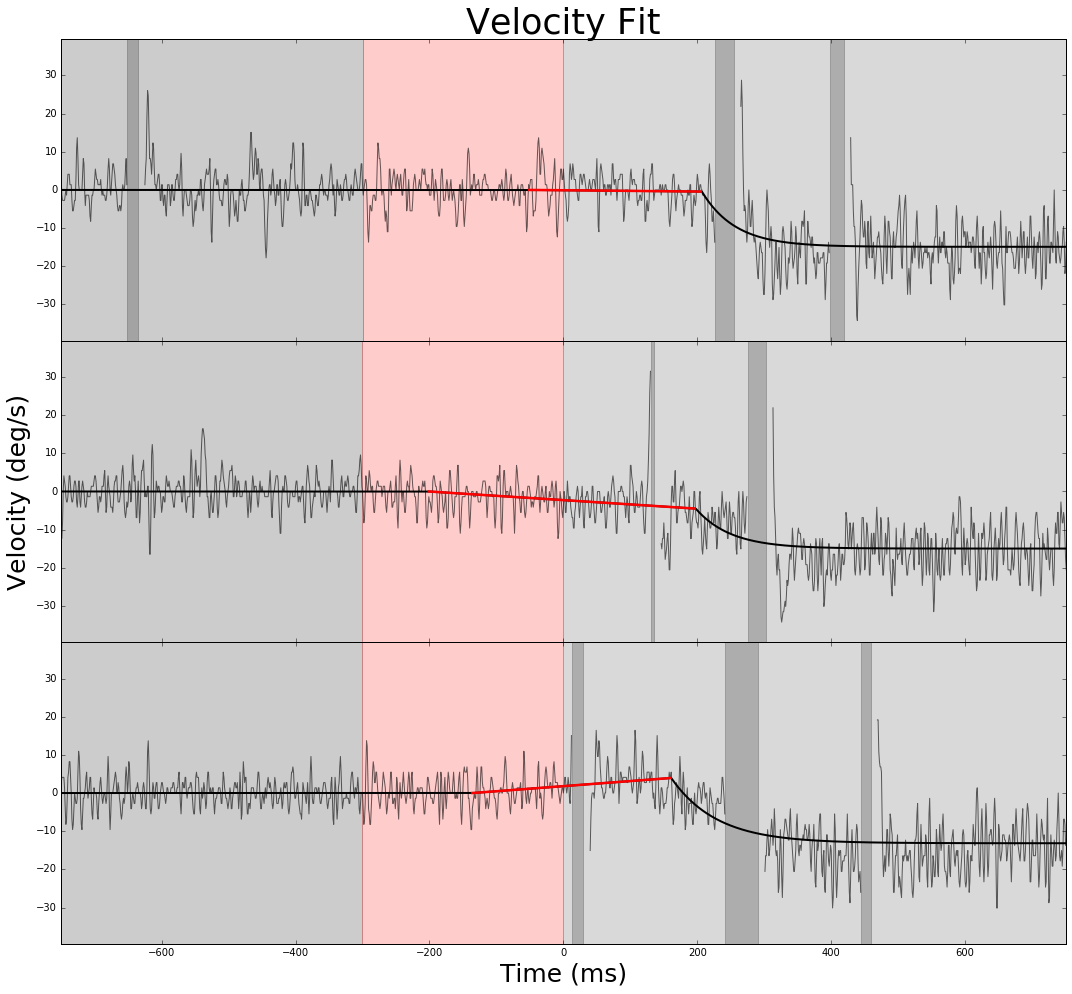
\includegraphics[width=1\columnwidth]{Fit_vitesse}
\end{center}

It is the acceleration of anticipation that we have extracted in order to compare it to the real probability :

\begin{center} 
    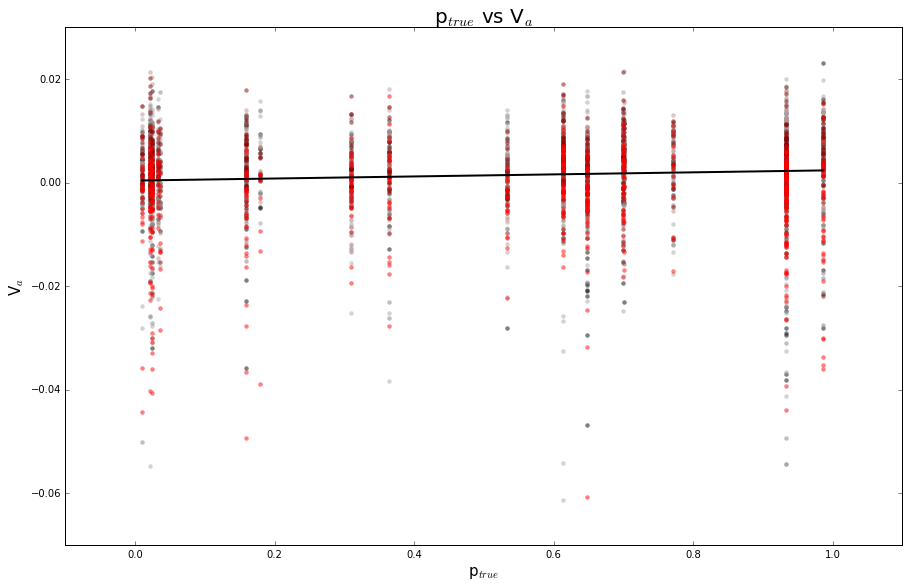
\includegraphics[width=1\columnwidth]{p_true--v_a}
\end{center}

\subsection*{<<Bet>> and <<Recording>>}

We now compare the probability bet during the bet with the acceleration of anticipation :

\begin{center} 
    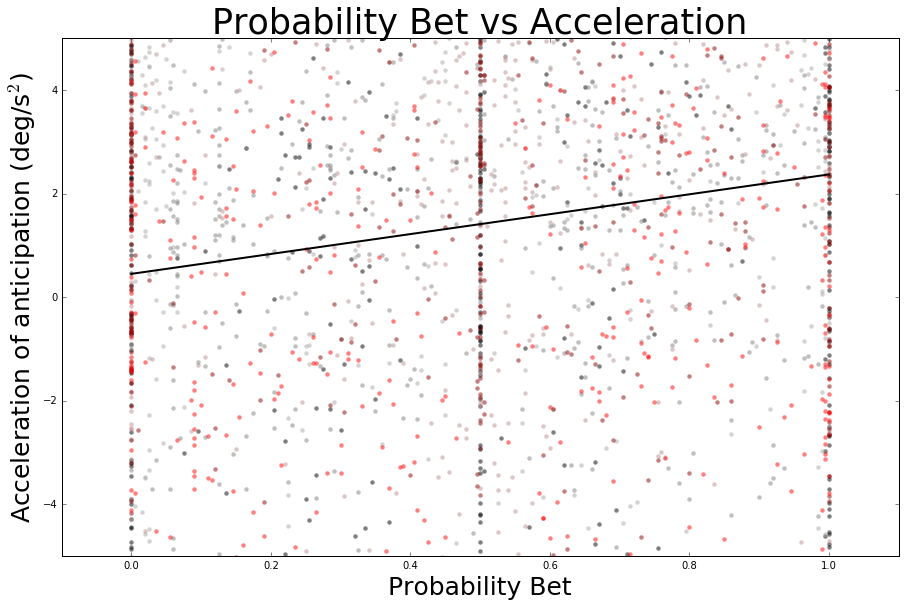
\includegraphics[width=1\columnwidth]{p_parie--v_a}
\end{center}

\section*{Conclusions}

...

{\small
\printbibliography
}
\end{multicols}


%%%%%%%%%%%%%%%%%%%%%%%%%%%%%%%%
\end{document}%
